%%%%%%%%%%%%%%%%%%%%%%%%%%%%%%%%%%%%%%%%%
%
% Original author:
% Philipp Stassen
%
% License:
% MIT https://mit-license.org/
%
%%%%%%%%%%%%%%%%%%%%%%%%%%%%%%%%%%%%%%%%%

%----------------------------------------------------------------------------------------
%	PACKAGES AND OTHER DOCUMENT CONFIGURATIONS
%----------------------------------------------------------------------------------------

%11pt is normal writing size
\documentclass[11pt]{scrartcl}


\usepackage[nochapters]{classicthesis} % Use the classicthesis style for the style of the document
\usepackage[LabelsAligned]{currvita} % Use the currvita style for the layout of the document
\usepackage[bottom=1cm, top=1.5cm, left=1cm, right=1cm, marginparsep=0.35in]{geometry}
\usepackage{paracol}
\usepackage{everypage}
\usepackage{graphicx}
\usepackage{tabularx}

\renewcommand{\cvheadingfont}{\LARGE\color{Orange}} % Font color of your name at the top

\usepackage{hyperref} % Required for adding links	and customizing them
\hypersetup{colorlinks, breaklinks, urlcolor=Orange, linkcolor=Orange} % Set link colors

%----------------------------------------------------------------------------------------
%	Setup columns with paracol 
%----------------------------------------------------------------------------------------

\columnsep=0.05\textwidth
\setcolumnwidth{.25\textwidth, .7\textwidth} 
\setlength{\columnseprule}{0.5pt}
\colseprulecolor{gray}

\tolerance=1                                                                                % Code fixes the justification issue with columns flowing over
\emergencystretch=\maxdimen                                                 %
\hyphenpenalty=10000                                                            %
\hbadness=10000  

%----------------------------------------------------------------------------------------
%	FONTS
%----------------------------------------------------------------------------------------

\usepackage[T1]{fontenc}
\usepackage{ebgaramond}
%\usepackage{roboto}
%\fontsize{11}{4}\selectfont

%----------------------------------------------------------------------------------------
%	FONT AWESOME ICONS
%---------------------------------------------------------------------------------------- 

% include the fontawesome icon set
\usepackage{fontawesome5}


%----------------------------------------------------------------------------------------
%	TABLE /ARRAY DEFINITIONS
%---------------------------------------------------------------------------------------- 

% extended aligning of tabular cells
\usepackage{array}

% custom column right-align with fixed width
% use like p{size} but via x{size}
\newcolumntype{x}[1]{%
>{\raggedleft\hspace{0pt}}p{#1}}%

%---------------------------------------------------------------------------------------- 
%	MACROS FÜR CV
%---------------------------------------------------------------------------------------- 

\NewDocumentCommand{\CVheader}{m}{{\Large\spacedlowsmallcaps{#1}}\\ \vspace{0.2cm}}
\NewDocumentCommand{\CVSubheader}{m}{{\spacedlowsmallcaps{#1}}}
\NewDocumentCommand{\CVentry}{m}{{{#1}}\\ \vspace{0.2em}}

%----------------------------------------------------------------------------------------
%	 CV EVENT
%----------------------------------------------------------------------------------------

% Manual aligning of tabular, because I don't know how to do it better
\newcommand{\LeftOffset}{-0.2cm}
\newcommand{\TopPadTabular}{0.1cm}


% param 1: time-frame i.e. Sep 14 - Jan 15 etc.
% param 2:	 event name (job position etc.)
% param 3: Customer, Employer, Industry
% param 4: Short description

\NewDocumentCommand{\CVevent}{mmmm}{
	% we wrap this part in a parbox, so title and description are not separated on a pagebreak
	% if you need more control on page breaks, remove the parbox
	\vspace{\TopPadTabular}
	\parbox{\linewidth}{
		\hspace{\LeftOffset}\begin{tabular*}{\linewidth}{p{0.8\linewidth}  r}
	 		{\raggedleft\spacedlowsmallcaps{#2}} & {\raggedleft{#1}} \\
			{\emph{#3}} 
		\end{tabular*}

		\vspace{0.2cm}

		{#4}
	}
	\vspace{0.1cm}
}

\NewDocumentCommand{\SBheader}{m}{{\Large\spacedlowsmallcaps{#1}}\\ \vspace{0.3em}}
\NewDocumentCommand{\SBSubheader}{m}{{\spacedlowsmallcaps{#1}}}
\NewDocumentCommand{\SBentry}{m}{{{#1}}\\ \vspace{0.2em}}

%----------------------------------------------------------------------------------------

%----------------------------------------------------------------------------------------
%	Remove Date 
%----------------------------------------------------------------------------------------

\date{}

\begin{document}

\thispagestyle{empty} % Stop the page count at the bottom of the first page

\begin{cv}{\centering\Huge\spacedallcaps{Dr. Philipp Stassen}} % Your name
	%---------- Horizontal Line ---------------------------%
	\vspace{0.5cm}
	\par\noindent\textcolor{gray}{\rule{\textwidth}{0.4pt}}

	%---------- First write on the left side, then, after "switchcolumn" on the right side

	\begin{paracol}{2}
		\begin{flushleft}
    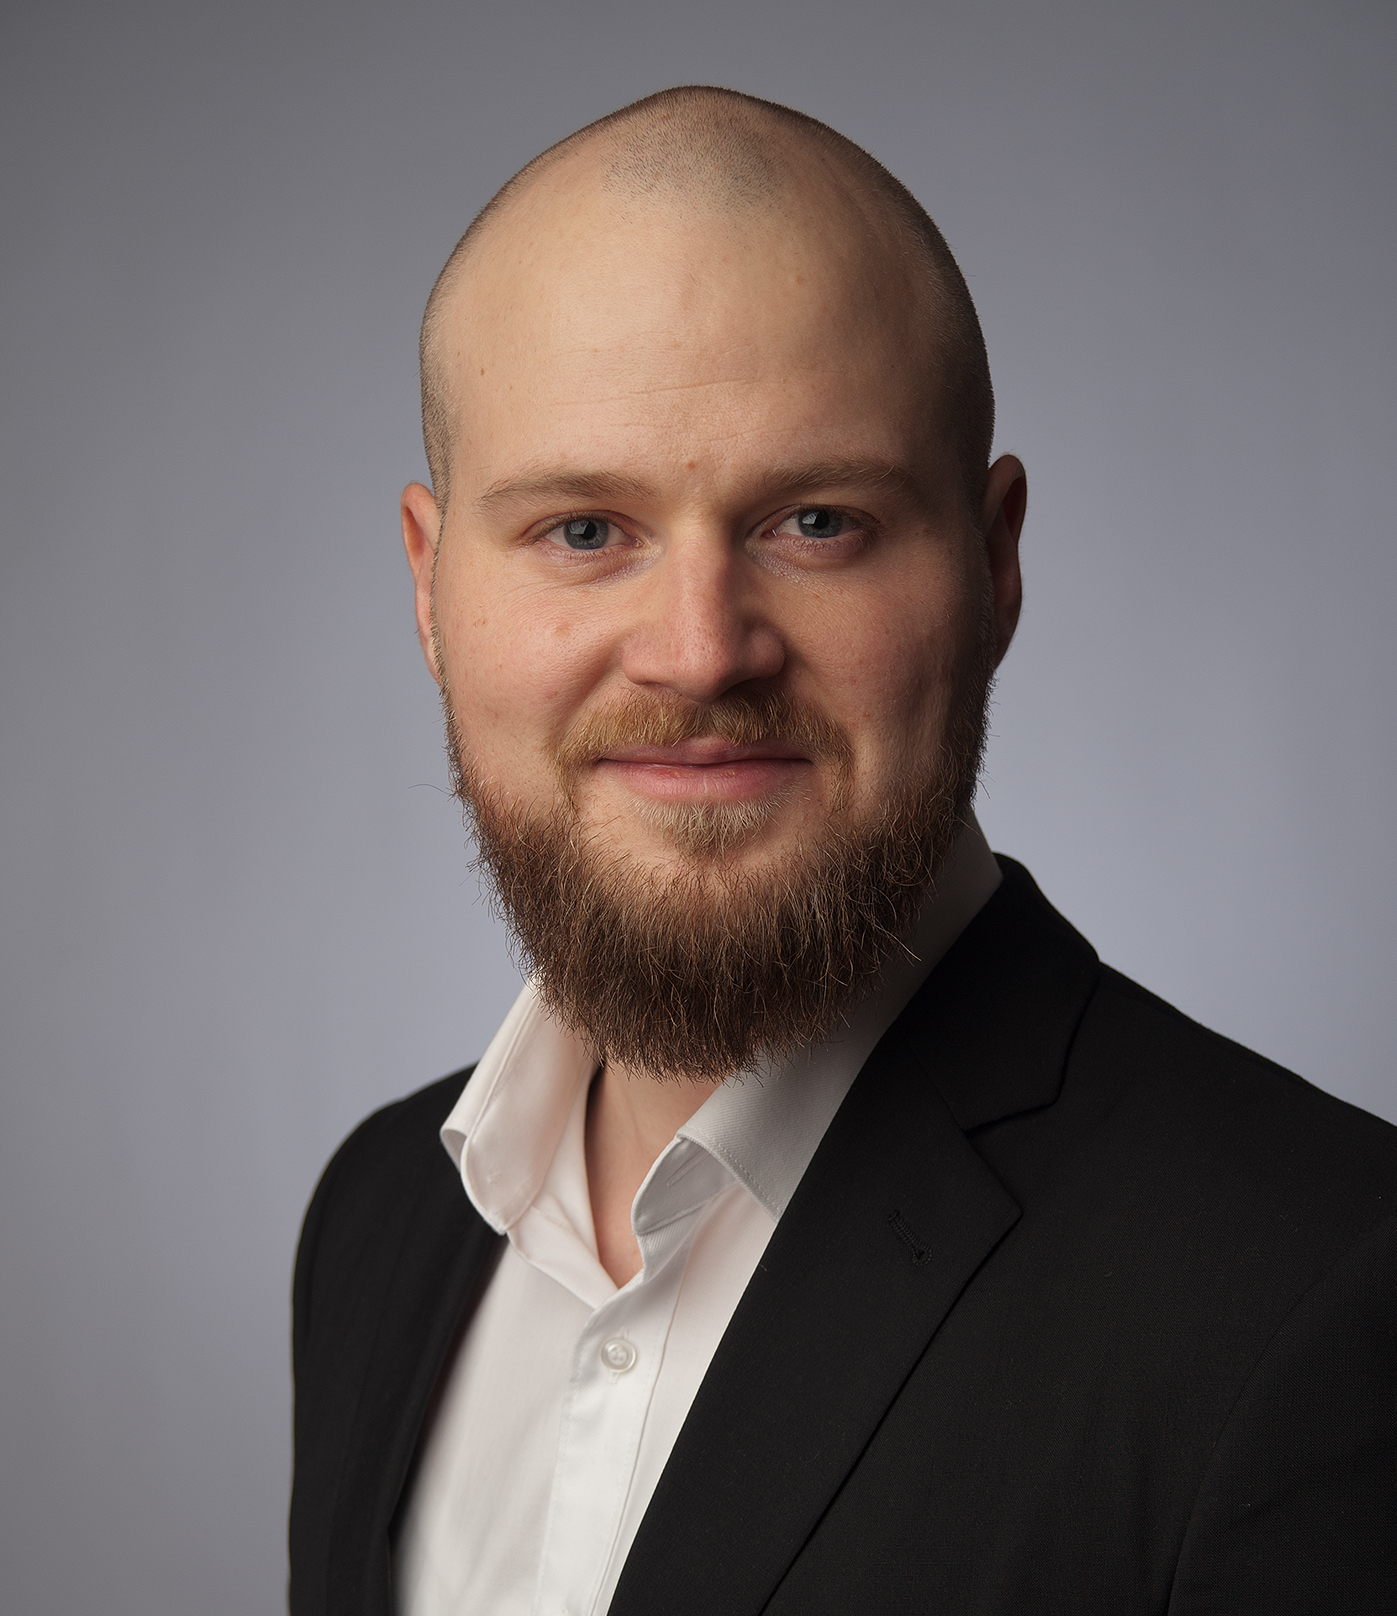
\includegraphics[scale=0.095]{photo} \\
	\vspace{0.4cm}
    \SBentry{Dr. Philipp Stassen}
	\SBentry{{\tiny \color{gray}\faStarOfLife}\ \ 31.01.1994 \ in Wiesbaden}
	\SBentry{{\small\color{gray}\faPhone}\ \ +49 160 5911912}
	\SBentry{{\small\color{gray}\faAt}\ \ philipp.stassen@gmail.com}
	\SBentry{{\small\color{gray}\faGlobe}\ \ www.philippstassen.github.io}

	\vspace{1cm}
	% ------------------------------------------------------------------------
	%	Skills
	% ------------------------------------------------------------------------
	\SBheader{Computer Skills}
		\SBentry{\SBSubheader{Programming}: OCaml, Haskell, Python, Agda, Shell, Html/CSS, LaTex}
		\SBentry{\SBSubheader{Software}: Coq, Emacs, Git, Iris, Mathematica, Docker}

	\vspace{1cm}
	% ------------------------------------------------------------------------
	%	Languages	
	% ------------------------------------------------------------------------
	\SBheader{Languages}
	\SBentry{\SBSubheader{Mothertongue}: German}
	\SBentry{\SBSubheader{Fluent}: English}
	\SBentry{\SBSubheader{Basic}: Spanish, Danish}

	\vspace{1cm}
	% ------------------------------------------------------------------------
	%	Contact field
	% ------------------------------------------------------------------------
	\SBheader{Contact} % Personal information heading
	\SBentry{Richard-Strauss-Str 23\\ 
	81677 Munich\\
	 Germany}

		\end{flushleft}
	\switchcolumn
	\begin{flushleft}
	\CVheader{About me}
	\CVentry{I am a computerscience PhD with strong theoretical and mathematical background. 
	My research centered around safety, security and semantics of programs. \\
	I am highly motivated to work in a team and as connecting or coordinating piece between various parties.
	My expertise, background knowledge and quick comprehension allow me lead and contribute on a multitude of topics.}

	\vspace{0.3cm}

	\CVSubheader{Expertise} \hspace{1em}
	\CVentry{Programming languages, Algorithms, Probabilistic programming, Program Verification, Machine Learning, Functional programming languages, Mathematical Modelling, Type Theories}

	\vspace{1cm}

	\CVheader{Experience}
	\CVevent{11.2022-04.2023}{PhD Residency}{Airbus Cyber Security}
	{Under the EU projects \emph{Albatross} and \emph{Concordia} Airbus Cyber Security contributed requirements and simulations to research projects which targeted the 
	safety and security standards of modern aviation.  \\
	\noindent
	\CVSubheader{Achievements:} We published the paper "Don’t Panic! Analysing the Impact of Attacks on the Safety of Flight Management Systems", which received the best paper award at DASC 2023
	}
	\CVevent{2022}{Conference Talk}{Types}{}
	\CVevent{2022}{Workshop talk}{WITS}{}
	\CVevent{2021\&2022}{Teaching assistant}{Computability and Logic}{}

	\vspace{1cm}
	\CVheader{Education}
	\CVevent{2020-06.2024}{PhD fellow}{Aarhus university, Department of Computer Science}{}
	\CVevent{2018 - 2020}{Master of Science}{Stockholm University, Mathematics}
	{
		\CVSubheader{Awards}: Mittag-Leffler prize
	}
	\CVevent{2014-2018}{Bachelor of Science}{University Bonn, Mathematics}{}
	\end{flushleft}

	%---------- Clearpage ensures that the vertical line is drawn to the end
	\clearpage
	\end{paracol}
\end{cv}
\end{document}

%\NewEntry{}{Born in Wiesbaden (Germany),}{31 January 1994} % Birthplace and date

%\NewEntry{address}{Richard-Strauss-Straße 23, 81677 München, Germany}

%\NewEntry{email}{\href{mailto:philipp.stassen@gmail.com}{philipp.stassen@gmail.com}} % Email address

%\NewEntry{website}{\href{https://www.philippstassen.github.io}{https://www.philippstassen.github.io}} % Personal website

%\NewEntry{phone}{+49 160 5911912} % Phone number(s)

%\NewEntry{nationality}{German}

%\vspace{2.7em} % Extra white space between the personal information section and goal

%%\noindent\spacedlowsmallcaps{Goal}\vspace{1em} % Goal heading, could be used for a quotation or short profile instead

%%\Description{Gain fundamental experience in my area of interest and expertise.}\vspace{2em} % Goal text

%%----------------------------------------------------------------------------------------
%\topic{Experience}

%\Description{\MarginText{Research Internship}2023\hspace{3.6em} Airbus Cyber Security

 	%\vspace{0.5em}
	%Publication: Don’t Panic! Analysing the Impact of Attacks on the Safety of Flight Management Systems 	
%}

%\Description{\MarginText{Conference Talks}2022\hspace{3.6em} {\textsc{TYPES}}\newline
  %2022\hspace{3.6em} {\textsc{WITS (POPL)}}\newline
%%  2019\hspace{3.6em} {\textsc{Proof, Computation and Complexity}}\newline
%%	2019 \hspace{3.3em} {\textsc{Mathematical Logic and Constructivity}} \newline
%%	2018 \hspace{3.3em} \textsc{Types, Sets and Constructions}
%%Developed spreadsheets for risk analysis on exotic derivatives on a wide array of commodities (ags, oils, precious and base metals), managed blotter and secondary trades on structured notes, liaised with Middle Office, Sales and Structuring for bookkeeping. \\ Reference: John \textsc{McDonald}\ \ $\cdotp$\ \ +1 (000) 111 1111\ \ $\cdotp$\ \ \href{mailto:john@lehman.com}{john@lehman.com}
%}

%%------------------------------------------------
%%
%%\NewEntry{2010--2011}{Summer Intern, \textsc{Initech Inc}  --- Chicago}
%%
%%\Description{\MarginText{Initech Inc}Rated "truly distinctive" for Analytical Skills and Teamwork. \\ Reference: Bill \textsc{Lumbergh}\ \ +1 (000) 111 1111\ \ $\cdotp$\ \ \href{mailto:bill@initech.com}{bill@initech.com}}
%%
%%------------------------------------------------

%%\NewEntry{2018}{\textsc{Preparation and tutelage of a course in mathematical logic}}

%\Description{\MarginText{Teaching}2021 \& 2022 \hspace{0.01em} Teaching Assistant: \textsc{Computability and Logic}\newline
  %2019 \hspace{3.3em} Preparation and tutelage of a course in \textsc{mathematical logic}
%%Worked in the Nerd Herd and helped to solve computer problems by asking customers to turn their computers off and on again. \\ Reference: Big \textsc{Mike}\ \ +1 (000) 111 1111\ \ $\cdotp$\ \ \href{mailto:mike@buymore.com}{mike@buymore.com}}
%}
%%------------------------------------------------

%\vspace{1em} % Extra space between major sections


%%----------------------------------------------------------------------------------------
%%	EDUCATION
%%----------------------------------------------------------------------------------------
%%\noindent\hspace{2em}\spacedlowsmallcaps{Education}\vspace{1em}
%\topic{Education}

%\Description{\MarginText{PhD} \hspace{-0.3em} 2020 - 2024 \hspace{0.7em} \textbf{Aarhus University, Denmark}

 	%\vspace{0.5em}
	%Department: Computer Science \newline
	%Thesis : Programming language semantics in modal type theories \newline
	%Defence : Friday 9 August 2024, Philipp Stassen \newline
%%Description: This thesis explored the idea that money has been the cause of untold anguish and suffering in the world. I found that it has, in fact, not.\newline
	%Supervisor: Prof. Lars Birkedal
%}

%%------------------------------------------------
%%\NewEntry{2018-2020}{Stockholm Universitet, Sweden}

%\Description{\MarginText{Master of Science} \hspace{-0.3em}2018-2020 \hspace{1em} \textbf{Stockholm Universitet, Sweden}
	
%%	\vspace{0.5em}
%%	Department: Mathematics \newline
%%	Thesis: \textit{An Analysis of Curien's Syntax for Dependent Type Theory}\newline
%%%Description: This thesis explored the idea that money has been the cause of untold anguish and suffering in the world. I found that it has, in fact, not.\newline
%%Supervisors: Assoc. Prof. Peter LeFanu \textsc{Lumsdaine} \& Dr. Guillaume \textsc{Brunerie}\newline
%%Grade: A \newline
%Awarded \textsc{Mittag-Leffler Prize}
%}

%%------------------------------------------------

%%\NewEntry{2014-2018}{Universität Bonn, Germany}

%\Description{\MarginText{Bachelor of Science}2014-2018 \hspace{1em} \textbf{Universität Bonn, Germany} 
%%
%%	\vspace{0.5em}
%%	\noindent Department: Mathematics\newline
%%Thesis: \textit{Formalism of homotopy type theory and its applications to logic} \newline
%%Supervisors: Prof. Peter \textsc{Koepke} \& Dr. Philipp \textsc{Lücke}\newline
%%Grade: 1.5
  %}


%%------------------------------------------------

%\vspace{1em} % Extra space between major sections

%%----------------------------------------------------------------------------------------
%%	WORK EXPERIENCE
%%----------------------------------------------------------------------------------------


%%	PUBLICATIONS
%%----------------------------------------------------------------------------------------

%%\spacedlowsmallcaps{Publications}\vspace{1em}
%%
%%\NewEntry{January 2013}{Publication Title}
%%
%%\Description{\MarginText{Full Journal Name}Lorem ipsum dolor sit amet, consectetur adipiscing elit. Ut nisl tellus, sodales non pulvinar in, adipiscing sit amet purus. Suspendisse sed facilisis diam. Sed ornare sem nec justo adipiscing nec venenatis lectus commodo. Mauris non neque ligula. Pellentesque sed quam eu felis iaculis iaculis ac a leo. Suspendisse neque neque, placerat id adipiscing et, elementum eu sem.\\ Authors: John \textsc{Smith}, ~James \textsc{Smith}}
%%
%%%------------------------------------------------
%%
%%\NewEntry{Sept. 2012}{Publication Title}
%%
%%\Description{\MarginText{Full Journal Name}Lorem ipsum dolor sit amet, consectetur adipiscing elit. Ut nisl tellus, sodales non pulvinar in, adipiscing sit amet purus. Suspendisse sed facilisis diam. Sed ornare sem nec justo adipiscing nec venenatis lectus commodo. Mauris non neque ligula. Pellentesque sed quam eu felis iaculis iaculis ac a leo. Suspendisse neque neque, placerat id adipiscing et, elementum eu sem.\\ Authors: John \textsc{Smith}, ~James \textsc{Smith}}
%%
%%------------------------------------------------

%%\vspace{1em} % Extra space between major sections

%%----------------------------------------------------------------------------------------
%%	COMPUTER SKILLS
%%----------------------------------------------------------------------------------------
%\topic{Computer Skills}

%\Description{\MarginText{Advanced} Agda, Vim, Emacs, OCaml}

%\Description{\MarginText{Intermediate} Github, Haskell, \LaTeX, Linux }

%\Description{\MarginText{Basic} C++, Coq, Iris, Mathematica, Python}

%%------------------------------------------------

%\vspace{1em} % Extra space between major sections

%\topic{Knowledge}

%\Description{\MarginText{Expert} Programming languages, Algorithms, Probabilistic programming, Program Verification, Machine Learning}
%%----------------------------------------------------------------------------------------
%%	OTHER INFORMATION
%%----------------------------------------------------------------------------------------

%%\topic{Awards}
%%
%%\Description{\MarginText{Mittag-Leffler} 2020 \hspace{3.3em} for my Master Thesis project}

%\topic{Languages}
%%\Description{\MarginText{Awards}2011\ \ $\cdotp$\ \ School of Business Postgraduate Scholarship}
%%
%%\vspace{-0.5em} % Negative vertical space to counteract the vertical space between every \Description command
%%
%%\Description{2010\ \ $\cdotp$\ \ Top Achiever Award -- Commerce}
%%
%%%------------------------------------------------
%%
%%\vspace{1em}
%%
%%\Description{\MarginText{Communication Skills}2010\ \ $\cdotp$\ \ Oral Presentation at the California Business Conference}
%%
%%\vspace{-0.5em} % Negative vertical space to counteract the vertical space between every \Description command
%%
%%\Description{2009\ \ $\cdotp$\ \ Poster at the Annual Business Conference in Oregon}
%%
%%------------------------------------------------

%\newlength{\langbox} % Create a new length for the length of languages to keep them equally spaced
%\settowidth{\langbox}{English} % Length equals the length of "English" - if you have a longer language in your list put it here

%\Description{\parbox{\langbox}{\textsc{German}}\ \ $\cdotp$\ \ \ Mothertongue}

%\vspace{-0.5em} % Negative vertical space to counteract the vertical space between every \Description command

%\Description{\parbox{\langbox}{\textsc{English}}\ \ $\cdotp$\ \ \ Fluent (written and spoken)}

%%\vspace{-0.5em} % Negative vertical space to counteract the vertical space between every \Description command
%%
%%\Description{\parbox{\langbox}{\textsc{Danish}}\ \ $\cdotp$\ \ \ Beginner }

%\vspace{1em} % Negative vertical space to counteract the vertical space between every \Description command
%------------------------------------------------

%\Description{\MarginText{Interests}Piano\ \ $\cdotp$\ \ Cooking\ \ $\cdotp$\ \ Running\ \ $\cdotp$\ \ Chess\ \ $\cdotp$\ \ Dancing}

%----------------------------------------------------------------------------------------
%25th April 2020
%
%\vspace{2em}
%\noindent Philipp Stassen
